\documentclass[11pt,a4paper]{article}

% ── Packages ──────────────────────────────────────────────
\usepackage[utf8]{inputenc}
\usepackage[T1]{fontenc}
\usepackage{amsmath,amssymb,amsfonts}
\usepackage{graphicx}
\usepackage{booktabs}
\usepackage{hyperref}
\usepackage{geometry}
\usepackage{caption}
\usepackage{subcaption}
\usepackage{float}

\geometry{margin=2.5cm}
\hypersetup{colorlinks=true,linkcolor=blue,citecolor=blue,urlcolor=blue}

% ── Title ─────────────────────────────────────────────────
\title{Monocular Visual Odometry on Low-Parallax Aerial Imagery:\\
       A Comparative Evaluation}
\author{Vasily Krukovsky}
\date{August 2026}

\begin{document}
\maketitle

% ══════════════════════════════════════════════════════════
\begin{abstract}
We build and evaluate a monocular visual odometry (VO) pipeline on the
ALTO aerial dataset, comparing three two-frame pose estimators: SIFT
with Essential-matrix decomposition, SIFT with Lucas--Kanade optical
flow, and SuperPoint\,+\,LightGlue. Hyperparameters are selected by grid
search on a held-out validation split, and results are reported on a
contiguous test segment. SuperPoint\,+\,LightGlue matches the classical
estimators on per-pair rotation accuracy, but its trajectory-level
drift is roughly an order of magnitude larger, driven by a small
number of severe pose failures rather than steady accumulation. We
trace these failures to low inter-frame parallax and a dropping
Essential-matrix inlier ratio, and show that the domain gap between
wide-baseline benchmark datasets (e.g.\ MegaDepth-1500) and
low-parallax, near-nadir aerial imagery reshapes the error
distribution, with translation-direction uncertainty becoming the
dominant term. We also report the computational footprint of each
approach on CPU/GPU.
\end{abstract}

% ══════════════════════════════════════════════════════════
\section{Mathematical Preliminaries}

\subsection{Two-View Geometry and Pose Recovery}
Given two calibrated views with intrinsics $K$ and a set of $N$
corresponding pixel coordinates
$\{(p_1^{(i)},\, p_2^{(i)})\}_{i=1}^{N}$, the Essential matrix $E$
satisfies the epipolar constraint
\begin{equation}
  \hat{p}_2^{(i)\top}\, E\, \hat{p}_1^{(i)} = 0,
  \qquad \hat{p} = K^{-1}p .
\end{equation}
$E$ factors as $E = [t]_{\times}R$, where $R \in SO(3)$ and
$t \in \mathbb{R}^3$ are the relative rotation and translation
direction.  We estimate $E$ using RANSAC
(\texttt{cv2.findEssentialMat}, confidence\,=\,0.999) and recover
$(R,t)$ via cheirality-checked SVD decomposition
(\texttt{cv2.recoverPose}).

\subsection{Degeneracy Check: Essential vs.\ Homography}
Because a purely planar scene or a purely rotational motion makes $E$
ill-defined, we additionally fit a homography $H$ and compare symmetric
transfer scores gated by a $\chi^2$ threshold:
\begin{equation}
  S_H = \sum_i \bigl[(\tau_H - e_{12}^{(i)})_+
                    + (\tau_H - e_{21}^{(i)})_+\bigr],
  \qquad
  S_F = \sum_i \bigl[(\tau_F - d_{12}^{(i)})_+
                    + (\tau_F - d_{21}^{(i)})_+\bigr],
\end{equation}
where $e_{12}, e_{21}$ are squared symmetric reprojection errors under
$H, H^{-1}$ ($\tau_H = 5.99$, 2~d.o.f., 95\%), and $d_{12}, d_{21}$
are squared point-to-epipolar-line distances under $F$
($\tau_F = 3.84$, 1~d.o.f., 95\%). This is the same model-selection
score ORB-SLAM uses during monocular initialization to flag
near-planar or near-degenerate scenes~\cite{orbslam}; we report it
here as a diagnostic ratio $R_H = S_H / (S_H + S_F + \varepsilon)$
rather than as a standalone measure of scene planarity.

\subsection{Correspondence Retention and Parallax}
For each pair we report the fraction of frame-1 keypoints that survive
to a valid correspondence after matching or tracking. We call this
\emph{correspondence retention} rather than repeatability: in the
multi-view geometry literature, repeatability is usually a property of
the detector alone (whether a keypoint is independently re-detected
under some geometric criterion), whereas the quantity here folds in
the matcher or tracker as well, and the exact acceptance criterion
differs by estimator --- Lowe's ratio test for SIFT+Essential,
optical-flow tracking success for SIFT+LK, LightGlue's learned match
confidence for SuperPoint+LightGlue. The three numbers are therefore
comparable as an end-to-end front-end yield, not as a shared
geometric property. Median parallax is the median angle, in the camera-1 reference frame,
between back-projected inlier bearing vectors:
\begin{equation}
  \theta_{\mathrm{par}}
    = \operatorname{median}_i
      \arccos\!\bigl(\hat{p}_1^{(i)\top}\hat{p}_2^{(i)}\bigr).
\end{equation}

\subsection{Pose Error, RPE and AUC@K}
The rotation error (degrees) is
\begin{equation}
  e_R = \arccos\!\left(\frac{\operatorname{tr}(R_{\mathrm{est}}
        R_{\mathrm{gt}}^{\top}) - 1}{2}\right)\frac{180}{\pi}.
\end{equation}
Since monocular translation is scale-free, the translation error is the
angle between unit directions:
\begin{equation}
  e_t = \arccos(\hat{t}_{\mathrm{est}} \cdot \hat{t}_{\mathrm{gt}})
        \frac{180}{\pi}.
\end{equation}
Following the evaluation protocol established for sparse matching on
MegaDepth-1500~\cite{lightglue,wang2026}, we report the Area Under the
recall Curve at threshold $K \in \{5^\circ, 10^\circ, 20^\circ\}$ of
the maximum angular pose error $e = \max(e_R, e_t)$:
\begin{equation}
  \mathrm{AUC@}K = \frac{1}{K}\int_0^K F(\theta)\,d\theta,
  \qquad
  F(\theta) = \frac{1}{N}\sum_{i=1}^{N}
              \mathbf{1}[e^{(i)} \le \theta].
\end{equation}

\subsection{Absolute Trajectory Error (ATE)}
Relative poses are chained into a trajectory $\{P_k\}$ and aligned to
ground truth via the Umeyama closed-form transform~\cite{umeyama}.  We
report two regimes: \emph{direction-only}, where GT scale is injected
at every step and the trajectory is aligned rigidly (SE(3), no scale
fit, since scale is already correct by construction); and
\emph{realistic}, where only the unit-norm translation direction is
estimated and a single global scale is fit post-hoc via full Sim(3)
alignment. Unqualified ``ATE'' elsewhere in this note refers to the
realistic/Sim(3) regime. To isolate the contribution of rare
catastrophic pairs from long-horizon drift, we also compute a
\textbf{Windowed ATE}, which re-initialises the chain every $W$ steps.

% ══════════════════════════════════════════════════════════
\section{Experimental Setup}

\paragraph{Dataset.}
We use a contiguous 200-frame segment of the ALTO dataset~\cite{alto} (downward-facing RGB video from a helicopter), 
split chronologically into train/val/test (40/30/30). It is important to note that the train split was utilized 
\emph{exclusively} during the initial development phase for pipeline debugging and sanity checks. 
It was not used for hyperparameter tuning, model training, or any form of data-driven optimization. 
All formal grid searches and final evaluations were conducted strictly on the validation and held-out test splits, respectively.

\paragraph{Camera Model.}

The camera intrinsic matrix is
\[
K =
\begin{pmatrix}
324.1 & 0 & 250.0 \\
0 & 324.1 & 250.0 \\
0 & 0 & 1.0
\end{pmatrix}.
\]

\subsection{Estimators and Hyperparameter Tuning}
We perform an exhaustive grid search on the validation split to select
hyperparameters that minimise the median of $\max(e_R, e_t)$.

\begin{table}[H]
\centering
\begin{tabular}{@{}lll@{}}
\toprule
\textbf{Estimator} & \textbf{Grid Searched} & \textbf{Selected} \\
\midrule
SIFT\,+\,Essential
  & \texttt{dist\_ratio} $\in \{0.6, 0.7, 0.8\}$
  & 0.8 \\
  & \texttt{ransac\_thresh} $\in \{0.5, 0.8, 1.0, 1.5, 2.0\}$
  & 0.5 \\
  & \texttt{nfeatures} $\in \{1000, 1500, 2000\}$
  & 2000 \\[4pt]
SIFT\,+\,LK
  & \texttt{nfeatures} $\in \{1000, 2000, 4000\}$
  & 1000 \\
  & \texttt{ransac\_thresh} $\in \{0.5, 0.8, 1.0, 1.5, 2.0\}$
  & 0.5 \\[4pt]
SuperPoint\,+\,LightGlue
  & \texttt{max\_keypoints} $\in \{1024, 2048\}$
  & 2048 \\
  & \texttt{ransac\_thresh} $\in \{0.5, 0.8, 1.0, 1.5, 2.0\}$
  & 0.5 \\
\bottomrule
\end{tabular}
\caption{Hyperparameter grids and selected values.}
\label{tab:hyperparams}
\end{table}

\paragraph{Note on RANSAC.}
The threshold interacts with the feature budget: at larger budgets,
higher thresholds consistently scored worse on the validation split.
We hypothesize this is because a looser threshold admits more
low-quality correspondences into the Essential-matrix estimate on
near-degenerate pairs, though we did not run a controlled ablation to
confirm this mechanism. The smallest threshold (0.5) was optimal, or
tied for best, for all three estimators.

% ══════════════════════════════════════════════════════════
\section{Results}

\subsection{Keypoint Stability and Matching Quality}

\begin{table}[H]
\centering
\begin{tabular}{@{}lccccc@{}}
\toprule
\textbf{Estimator} & \textbf{Retent.} & \textbf{Inlier (E)} & \textbf{F Inlier} & \textbf{H Inlier} & $R_H$ \\
\midrule
SIFT\,+\,Essential       & 0.634 & 0.916 & 0.884 & 0.522 & 0.595 \\
SIFT\,+\,LK              & 0.968 & 0.962 & 0.941 & 0.627 & 0.599 \\
SuperPoint\,+\,LightGlue & 0.730 & 0.639 & 0.630 & 0.284 & 0.586 \\
\bottomrule
\end{tabular}
\caption{Correspondence retention and RANSAC-verified matching quality (mean over 56 test pairs).}
\label{tab:matching}
\end{table}

SIFT\,+\,LK retains the largest fraction of correspondences (0.968)
and has the highest Essential-matrix inlier ratio. $R_H$ sits in a
narrow 0.586--0.599 band across all three estimators, which we read as
a property of the scene --- the near-nadir, relatively flat ALTO
terrain --- rather than of the front end.

\subsection{Pose Accuracy and Comparison with State-of-the-Art}

\begin{table}[H]
\centering
\resizebox{\textwidth}{!}{
\begin{tabular}{@{}lcccccc@{}}
\toprule
\textbf{Estimator}
& $e_R$ med.\ ($^\circ$) & $e_t$ med.\ ($^\circ$)
& AUC@5$^\circ$ & AUC@10$^\circ$ & AUC@20$^\circ$
& Acc.@20$^\circ$ \\
\midrule
SIFT\,+\,Essential       & 0.177 & 9.791 & 0.017 & 0.107 & 0.501 & 96.4\% \\
SIFT\,+\,LK              & 0.139 & 10.398 & 0.000 & 0.085 & 0.493 & 98.2\% \\
SuperPoint\,+\,LightGlue & 0.275 & 11.857 & 0.022 & 0.104 & 0.377 & 76.8\% \\
\emph{LightGlue~\cite{lightglue} (MegaDepth-1500)}
& --- & --- & 0.561 & 0.717 & 0.828 & --- \\
\bottomrule
\end{tabular}
}
\caption{Relative Pose Error and AUC@$K$ (test split, gap\,=\,5).}
\label{tab:pose}
\end{table}

\paragraph{Domain Gap Analysis.}
The AUC@$K$ metrics on ALTO fall well short of the MegaDepth-1500
baseline reported in the LightGlue paper~\cite{lightglue}, and we
attribute the gap to scene geometry rather than to matcher quality.
MegaDepth is dominated by diverse, high-parallax scene pairs where
translation direction is well constrained; ALTO's near-nadir views
have a small baseline relative to scene depth, so translation
direction is comparatively hard to pin down ($e_t$ median
$\approx 9.8^\circ$--$11.9^\circ$ across the three estimators). Since
the AUC protocol takes $e = \max(e_R, e_t)$, this alone caps AUC@20 at
roughly 50\% for both SIFT variants, regardless of their rotational
accuracy.

\subsection{Geometric Analysis: Drift and Absolute Trajectory Error}

\begin{table}[H]
\centering
\resizebox{\textwidth}{!}{
\begin{tabular}{@{}lccc@{}}
\toprule
\textbf{Estimator}
& \textbf{ATE, dir.-only (m / \%)}
& \textbf{ATE, realistic (m / \%)}
& $s^\star$ \\
\midrule
SIFT\,+\,Essential       & 0.042 / 0.35\% & 0.041 / 0.34\% & 1.00 \\
SIFT\,+\,LK              & 0.031 / 0.26\% & 0.031 / 0.26\% & 1.00 \\
SuperPoint\,+\,LightGlue & 1.019 / 8.49\% & 0.730 / 6.08\% & 1.24 \\
\bottomrule
\end{tabular}
}
\caption{ATE over a 12.0\,m ground-truth test-split segment (gap\,=\,5).}
\label{tab:ate}
\end{table}

\begin{table}[H]
\centering
\resizebox{\textwidth}{!}{
\begin{tabular}{@{}lccc@{}}
\toprule
\textbf{Estimator} & \textbf{Median Latency (ms)} & \textbf{Median CPU RAM (MB)} & \textbf{Median GPU VRAM (MB)} \\
\midrule
SIFT\,+\,Essential       & 279.6 & 27.6 & 0.0 \\
SIFT\,+\,LK              & 108.6 & 22.8 & 0.0 \\
SuperPoint\,+\,LightGlue & 198.8 & 0.0  & 532.6 \\
\bottomrule
\end{tabular}
}
\caption{Computational footprint per pair estimation (measured on CPU/GPU; 5 pairs $\times$ 5 runs each, one representative profiling pass --- absolute latency varies by a few percent run to run, ranking is stable).}
\label{tab:compute}
\end{table}

\begin{figure}[H]
\centering
\begin{subfigure}[b]{0.48\textwidth}
  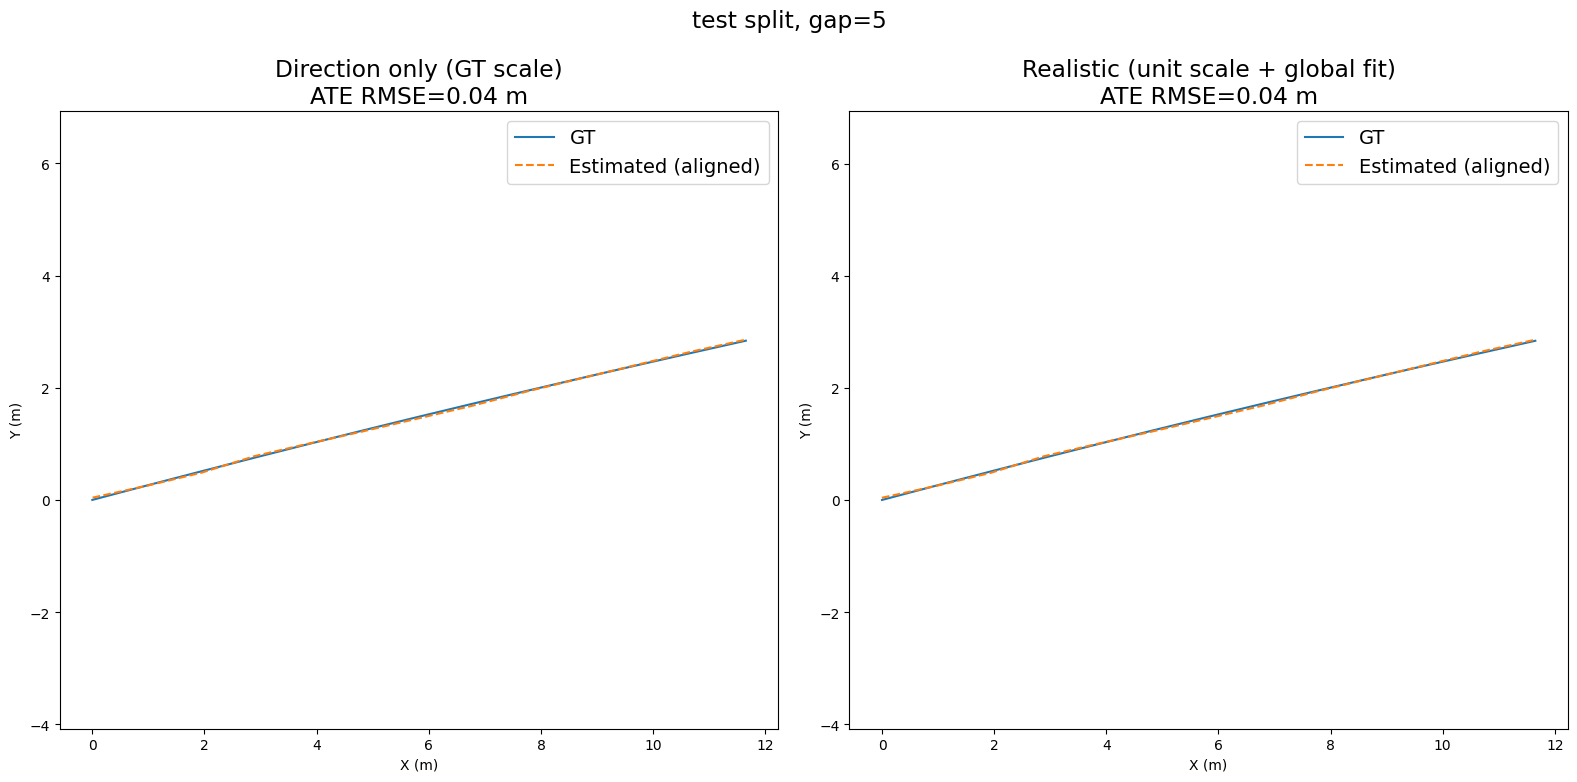
\includegraphics[width=\textwidth]{../figures/generated/fig_ate_sift_essential.png}
  \caption{SIFT\,+\,Essential}
\end{subfigure}
\hfill
\begin{subfigure}[b]{0.48\textwidth}
  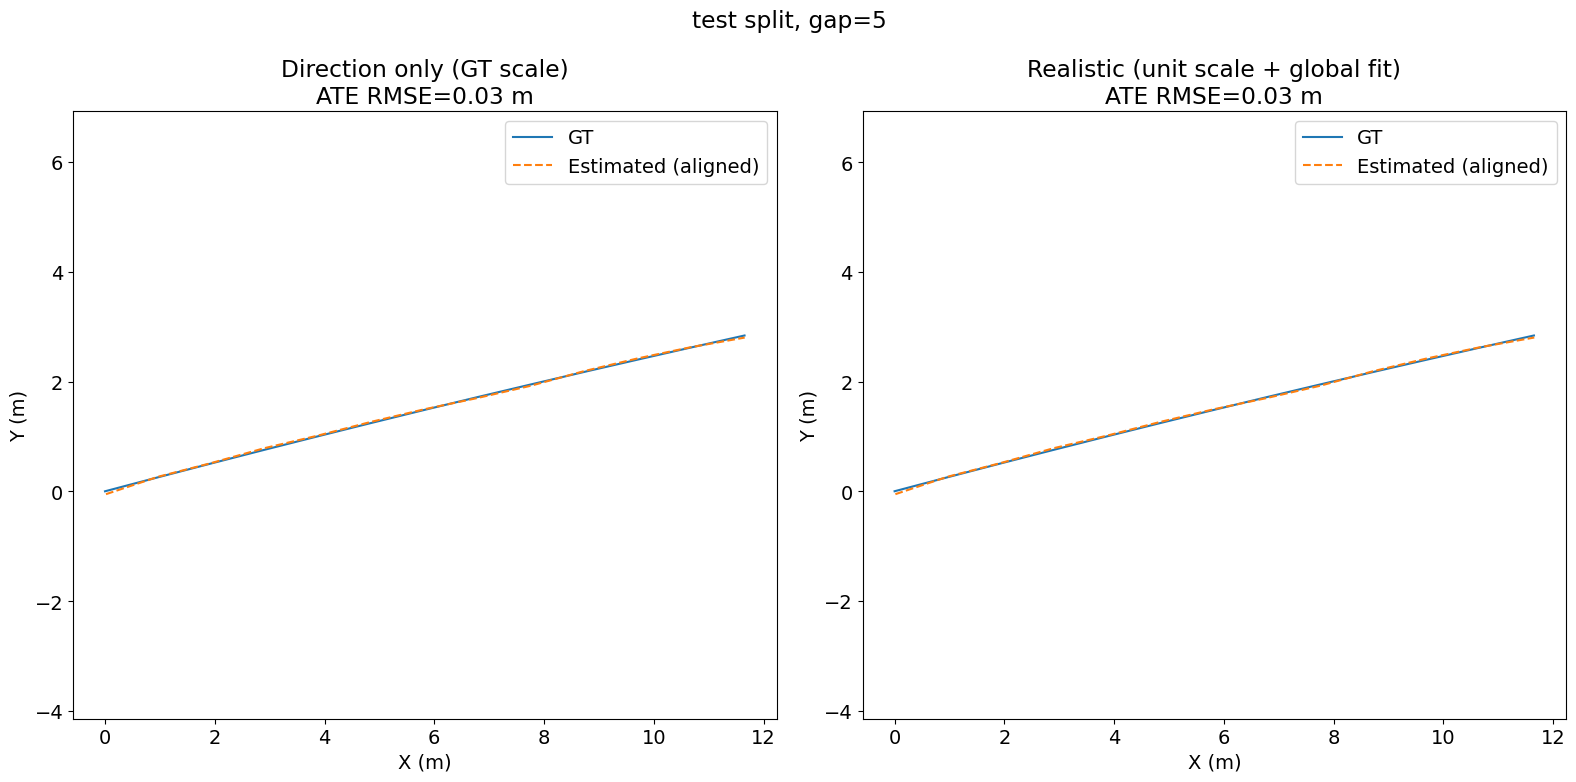
\includegraphics[width=\textwidth]{../figures/generated/fig_ate_sift_lk.png}
  \caption{SIFT\,+\,LK}
\end{subfigure}

\medskip
\begin{subfigure}[b]{0.48\textwidth}
  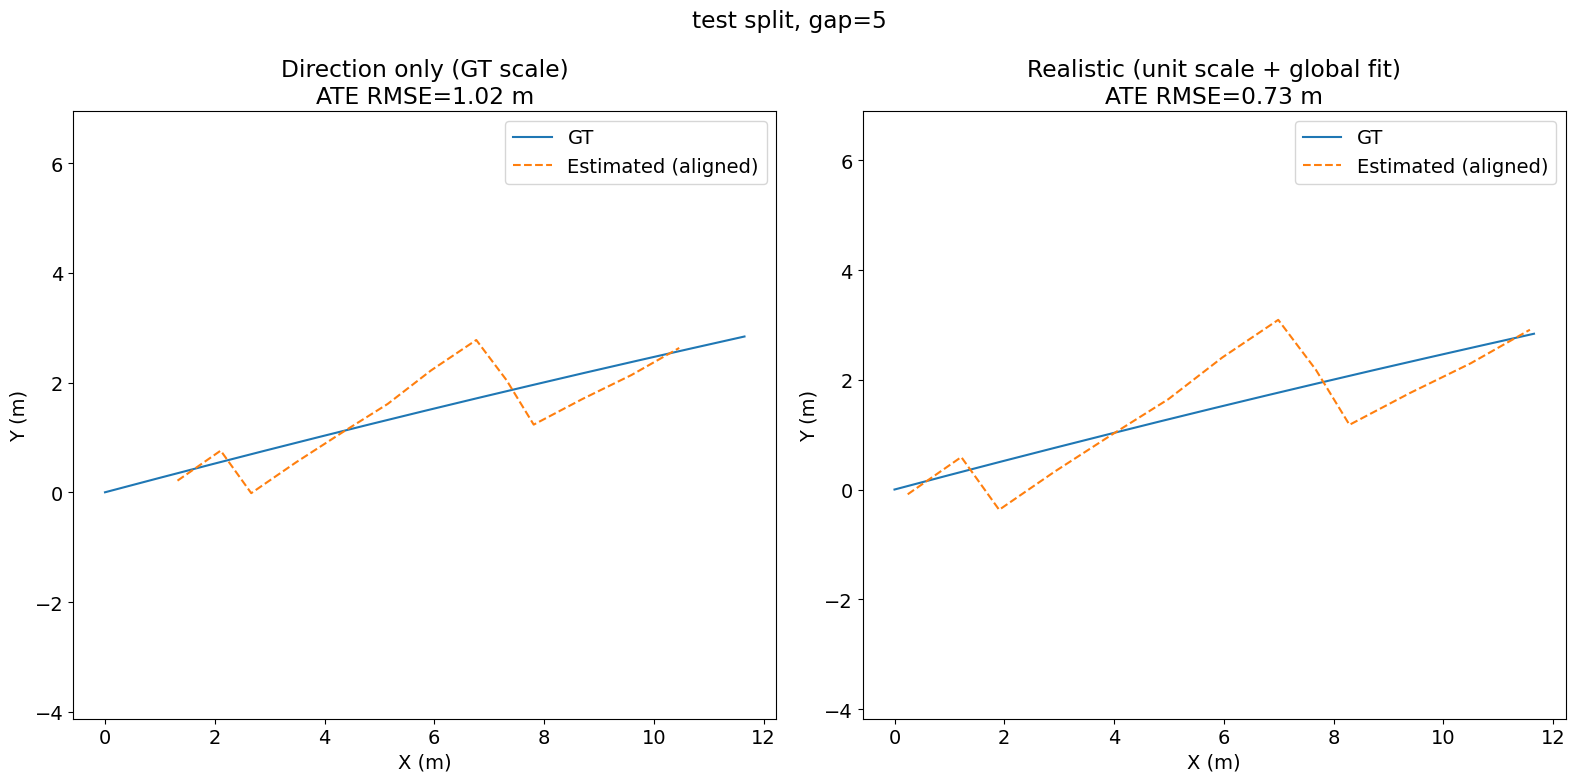
\includegraphics[width=\textwidth]{../figures/generated/fig_ate_superpoint_lg.png}
  \caption{SuperPoint\,+\,LightGlue}
\end{subfigure}
\caption{Estimated vs.\ ground-truth trajectory (direction-only, left
  panels; realistic scale, right panels).  Both SIFT variants overlay
  almost perfectly on the GT, while SuperPoint\,+\,LightGlue exhibits a
  sharp discontinuity early in the sequence.}
\label{fig:trajectories}
\end{figure}

SuperPoint\,+\,LightGlue matches the classical estimators on per-pair
rotation accuracy (Table~\ref{tab:pose}), yet accumulates roughly
$18\times$ more absolute trajectory error under the realistic
(Sim(3)) alignment, and roughly $24\times$ more under the
direction-only alignment (Table~\ref{tab:ate}). The trajectory plots
show why: this is not steady drift but a single severe mis-estimation
early in the chained sequence that permanently offsets everything
downstream of it.


% ══════════════════════════════════════════════════════════
% ══════════════════════════════════════════════════════════
\section{Discussion}

\paragraph{Estimator Selection and Computational Footprint.}
Among the methods evaluated on this ALTO test segment, SIFT\,+\,LK is
the best choice: lowest relative ATE (0.26\%), highest correspondence
retention (0.968), lowest median latency (108.6\,ms), CPU-only, no
VRAM. SIFT\,+\,Essential trails slightly on accuracy and costs more
compute (279.6\,ms median). SuperPoint\,+\,LightGlue needs a GPU and
532.6\,MB of VRAM, and on this dataset that cost buys no accuracy
advantage --- if anything, it is more exposed than either classical
estimator to the low-parallax degeneracies characteristic of
near-nadir aerial imagery. We would not generalize this ranking beyond
low-parallax, near-nadir aerial footage without re-running the same
protocol on a dataset with more viewpoint diversity.

\paragraph{The Translation Direction Bottleneck.}
The comparison with the LightGlue paper matters mainly as a warning:
standard sparse-matching metrics such as AUC@$K$ can be misleading on
near-nadir trajectories. The epipolar geometry in this setup produces
nearly parallel epipolar lines, so translation direction becomes
sensitive to sub-pixel feature-localisation error in a way that has
little to do with matcher quality. This caps AUC@20 near 50\% for both
classical methods regardless of their rotational accuracy, so AUC@$K$
alone would rank all three estimators as mediocre even though two of
them reconstruct the trajectory almost exactly.

\paragraph{Failure-Rate Analysis and Geometric Degeneracy.}
To rigorously evaluate robustness, we define a failure as a pair where $e_R > 2^\circ$ or $e_t > 20^\circ$. 
Under these thresholds, SIFT\,+\,LK exhibits a failure rate of only 1.79\% (1 out of 56 pairs), 
and SIFT\,+\,Essential 3.57\% (2 pairs). In stark contrast, SuperPoint\,+\,LightGlue fails in 23.21\% 
of cases (13 out of 56 pairs). 

As a diagnostic rather than a causal test, we compute the Spearman
rank correlation $\rho$ between the maximum pose error
$e = \max(e_R, e_t)$ and each geometric diagnostic, restricted to
SuperPoint\,+\,LightGlue:
\begin{equation}
\rho = 1 - \frac{6 \sum_{i=1}^{n} d_i^2}{n(n^2 - 1)}
\end{equation}
where $d_i$ is the difference in ranks between the pose error and the
diagnostic metric. We find moderate-to-strong negative correlations,
$\rho(e, \text{parallax}) = -0.64$ and $\rho(e, \text{inlier\_ratio}) =
-0.48$; with $n = 56$ pairs and only 13 flagged failures, we treat
these as suggestive rather than conclusive, and do not report a
significance test here (see Limitations). Together with the
trajectory plots, they are consistent with SuperPoint\,+\,LightGlue's
failures concentrating on low-parallax, low-inlier-ratio frames --- a
condition that recurs in low-altitude, straight-flight aerial
segments --- rather than with the scene-planarity statistic $R_H$,
which does not separate the failure cases (Table~\ref{tab:matching}
already shows $R_H$ barely varies across estimators). SIFT\,+\,LK is
noticeably more resilient on the same pairs.

% ══════════════════════════════════════════════════════════
% ══════════════════════════════════════════════════════════
\section{Limitations and Future Work}
\begin{enumerate}
\item \textbf{Unknown Camera-to-Sensor Extrinsic Calibration.}
The ground-truth poses are derived from an onboard navigation sensor (e.g., GPS/INS), 
whereas the visual odometry pipeline estimates the camera pose. The rigid body 
transformation (extrinsic calibration) between the camera optical center and the navigation sensor 
frame is not provided in the dataset. This uncalibrated offset introduces a systematic bias, 
particularly affecting the translation estimates, as the measured translation vector is contaminated 
by the lever-arm effect during rotational movements. Accounting for this extrinsic offset would likely reduce 
the residual translation bias further, though we have not established what accuracy floor is actually reachable 
on this dataset once it is corrected for.

\item \textbf{Statistical Power of Rare Events.}
The test split yields 56 overlapping pairs. While sufficient to evaluate median drift and windowed ATE, 
this sample size limits the statistical power of rare-event analysis. For instance, SuperPoint\,+\,LightGlue 
exhibited 13 catastrophic failures under the thresholds $e_R > 2^\circ$ or $e_t > 20^\circ$, corresponding 
to a failure rate of 23.21\%. We treat this as a diagnostic indicator of geometric degeneracy under low parallax 
rather than a rigorous, population-level statistic. A larger, more diverse aerial dataset is required to 
confidently quantify the tail of the error distribution.

\item \textbf{Absence of Fine-Tuning on the Train Split.}
As noted in the experimental setup, the 79-frame train split was reserved solely for code development. 
All three estimators utilise classical or frozen pretrained pipelines without any adaptation to the target 
domain. Fine-tuning the LightGlue attention mechanism on the ALTO train split could potentially adapt the 
matcher to the specific texture and parallax characteristics of aerial nadir views.

\item \textbf{RANSAC Variants.}
We utilised standard RANSAC. Evaluating LO-RANSAC or MAGSAC++ could further isolate how much of the 
remaining AUC gap is attributable to the robust estimation backend versus the feature front-end.
\end{enumerate}

% ══════════════════════════════════════════════════════════
\begin{thebibliography}{9}

\bibitem{alto}
I.~Cisneros, P.~Yin, J.~Zhang, H.~Choset, S.~Scherer.
\newblock ALTO: A Large-Scale Dataset for UAV Visual Place Recognition and
  Localization.
\newblock \emph{arXiv:2207.12317}, 2022.

\bibitem{lightglue}
P.~Lindenberger, P.-E.~Sarlin, M.~Pollefeys.
\newblock LightGlue: Local Feature Matching at Light Speed.
\newblock \emph{ICCV}, 2023.

\bibitem{wang2026}
Q.~Wang.
\newblock Understanding and Optimizing Attention-Based Sparse Matching for
  Diverse Local Features.
\newblock \emph{arXiv:2602.08430}, 2026.

\bibitem{umeyama}
S.~Umeyama.
\newblock Least-Squares Estimation of Transformation Parameters Between Two
  Point Patterns.
\newblock \emph{IEEE TPAMI}, 13(4), 1991.

\bibitem{orbslam}
R.~Mur-Artal, J.M.M.~Montiel, J.D.~Tard\'{o}s.
\newblock ORB-SLAM: A Versatile and Accurate Monocular SLAM System.
\newblock \emph{IEEE Transactions on Robotics}, 31(5), 2015.

\end{thebibliography}

\end{document}